\chapter{Marco teórico}

En este capitulo, se introducen conceptos básicos sobre robots y sus componentes.

La primera sección describe al robot industrial utilizado y sus componentes de hardware.

Finalmente se hace una breve descripción de distintos componentes de software utilizados.


\section{Manipulador robótico}



\subsection{Tipos de manipuladores}

\subsection{Características Scorbot ER VII}

El Scorbot-ER VII es un  manipulador robótico de cinco grados de libertad (5 DOF) diseñado para propósitos educacionales. Posee la configuración estándar de robot industrial antropomórfico (Figura \ref{cap2_scorbot}), ie. \textit{base}, \textit{shoulder} y \textit{elbow}.

\begin{figure}[ht]
  \centering
  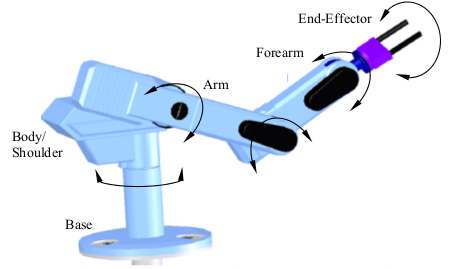
\includegraphics[scale=0.5]{img/cap2/scorbot}
  \caption{Scorbot-ER VII.}
  \label{cap2_scorbot}
\end{figure}

El sistema de actuación del robot se basa en el uso de poleas reductoras seguidas de engranajes armónicos (\textit{harmonic drives}) actuados por motores de corriente continua de imanes permanentes de una corriente máxima de \SI{18}{\ampere} a \SI{24}{\volt}. La carga máxima que puede llevar el robot es de \SI{2}{\kilo\gram} (incluido el peso del efector). Esta configuración asegura que el sistema es relativamente seguro para operar fuera de una jaula de seguridad \cite{scorbot1998}.

\section{Conceptos de cinemática}

Una de las tareas principales de un robot manipulador corresponde a seguir una trayectoria dejando al efector en una posición deseada. En orden de mover el robot a través de dos o más puntos de una trayectoria objetivo en un tiempo, velocidad y aceleración especificados, es necesario definir el movimiento de cada uno de los componentes del robot.

El análisis cinemático es el estudio del movimiento de los distintos elementos del robot, sin considerar las fuerzas y momentos que producen tal movimiento de los elementos.

\subsection{Cinemática directa}

Cinemática directa es el nombre que recibe el problema de encontrar la posición y orientación del efector relativo a la base del robot dados todas posiciones de las articulaciones y parámetros geométricos de los elementos que constituyen el robot. Usualmente, el sistema de referencia fijo en el efector se denomina \textit{tool frame} \cite{handbook}.

En la práctica, la cinemática directa es resuelta notando que para una cadena de elementos en serie, como es el caso del robot Scorbot, la transformada entre el sistema de referencia y el sistema fijo en el efector esta dada por la concatenación de las transformadas entre elementos adyacentes de la cadena cinemática.

\begin{equation}
T_0^5(\vec{\theta}) = T_0^1 T_1^2 T_2^3 T_3^4 T_4^5 
\end{equation}

Donde $\vec{\theta}=[\theta_1,\dotsc,\theta_5]$, $\theta_i$ corresponde al ángulo de la articulación $i$-ésima y $T_j^i$ es la transformada homogénea del elemento $i$ con respecto al sistema de referencia $j$.

\subsection{Cinemática inversa}

Por otro lado, la cinemática inversa es el nombre que recibe el problema de encontrar el valor de las posiciones de las articulaciones dada la posición y orientación del efector.
Usualmente, el cálculo de la cinemática inversa involucra la resolución de sistemas geométricos complejos que dificulta la obtención de formas cerradas, en casos donde la forma cerrada no existe se pueden emplear métodos numéricos basados en el jacobiano del sistema.

La obtención de modelos exactos de cinemática directa e inversa es tratado de forma extensa en \cite{cole2007} y \cite{predescu2015}.

\section{Control de motores DC}

\subsection{Sistemas electrónicos involucrados}

\subsection{Concepto de tiempo real}

\subsection{Buses de campo}

\section{Interfaces hápticas}

Los dispositivos hápticos son capaces de proporcionar una retroalimentación de fuerza al usuario que lo emplea, de esta forma, complementan sistemas de operación visuales al entregar más información al operador. Esta tecnología puede aplicarse a múltiples sectores con el fin de facilitar su ejecución: medicina, realidad virtual, modelado, robótica, entre otras.

\subsection{Phantom Omni}

Phantom Omni es un dispositivo háptico de seis grados de libertad (6 DOF) desarrollado por Sensable, permite leer la posición de sus seis articulaciones y posee tres actuadores conectados a los tres primeras articulaciones, permitiendo la aplicación de fuerzas, que solo pueden controlar la posición del \textit{stylus} en el espacio cartesiano.

\begin{figure}[ht]
  \centering
  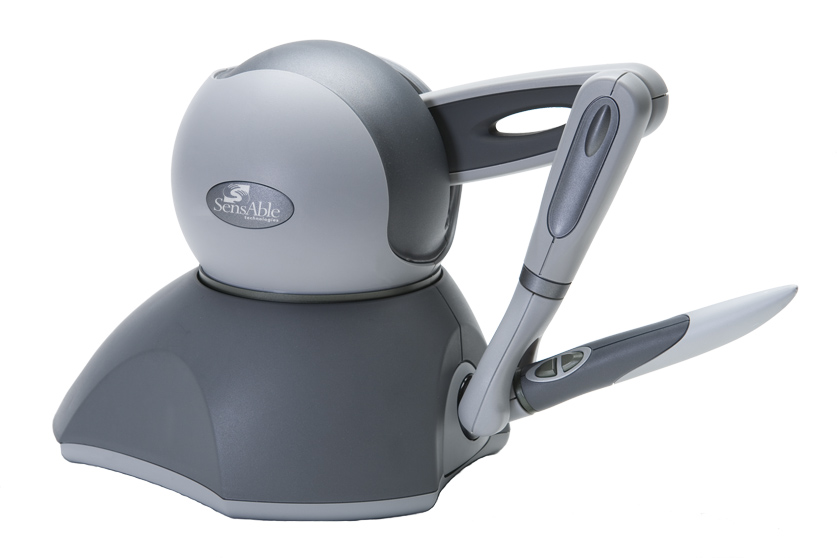
\includegraphics[scale=.2]{img/cap2/phantom_omni}
  \caption{Phantom Omni.}
  \label{cap2_phantom}
\end{figure}

Un aspecto importante del diseño es el desacople entre la posición y orientación \cite{beckman2007}, las tres primeras articulaciones son usadas para posicionar el \textit{stylus} y las restantes establecen la orientación del mismo. Los ejes de giro de estas últimas tres articulaciones se intersectan en un mismo punto, por lo que se puede interpretar como una articulación esférica.


\section{Componentes de software}

\subsection{ROS}

Hola esto es una cita a ROS \cite{quigley2009}.



Esto es una cita a TF \cite{foote2013}.

cita a Orocos \cite{orocos2001}

\cite{craig1989}

\cite{gier2015}

\cite{diankov2010}

